To be able to use the governance rules to manage the project we need to: (1) provide support for the recording of the information generated by all the participants interactions (e.g., proposals, votes, etc.), and (2) implement a decision engine that can use this information and apply the governance rules to make the corresponding decisions. 

To record the participant's interactions we use the schema shown in Figure \ref{fig:collaboration}. A particular collaboration (\texttt{Collaboration} metaclass) is represented by an identifier (\texttt{id} attribute) and a rationale explaining the collaboration (\texttt{rationale} attribute). There are three types of collaboration elements (\texttt{type} attribute in \texttt{Collaboration} metaclass): tasks, which represent a request for an issue or a bug; patches, which represent the solution for a task; and comments, which represent comments that users can make to other collaborations. A collaboration element can also have some metadata information (\texttt{metadata} reference) and has a proposing user (\texttt{isProposed} reference) and a leader (\texttt{leader} reference). During the collaboration, a user (\texttt{User} metaclass) is identified by an identifier (\texttt{id} attribute) and belongs to a one or more roles (\texttt{roles} reference).  Note also that both collaboration elements and users are linked to the tracking system (see \texttt{Tracking System} component) to retrieve the information of tasks/patches/comments and users, respectively. The metamodel also allows representing votes (\texttt{Vote} metaclass) from the users, which can agree/disagree with a collaboration (\texttt{agreement} attribute). A vote has a timestamp (\texttt{timeStamp} attribute) and a rationale (\texttt{rationale} attribute) explaining the reason for the positive/negative vote. 


\begin{figure*}[!t] 
  \centering
  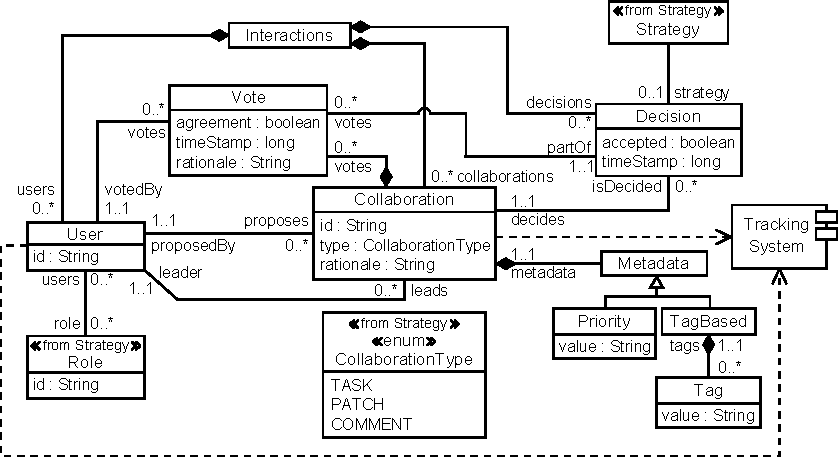
\includegraphics[width=0.8\textwidth]{./figures/collaboration}
  \caption{Metamodel to represent collaborations.}
  \label{fig:collaboration}
\end{figure*}

When the deadline for a governance rule passes, the decision engine receives the collaboration model as input and follows the rule instructions to process the data and take a decision. The decision updates the collaboration information to create the new decisions (\texttt{Decision} metaclass) and trace them back to the affected collaboration elements (\texttt{isDecided} reference). A decision can accept/reject a collaboration element (\texttt{accepted} attribute), includes a timestamp of the moment when the decision was made (\texttt{timeStamp} attribute) and refers to the strategy applied (\texttt{strategy} reference). A collaboration element has usually only decision element assigned except when a phased strategy is used, in this case the decisions for each phase and the final decision are also stored in the model. The decision engine is provided as part of our prototype tool implementation (see Section \ref{sec:implementation}).

